  {\large \fontB Description:}
  
  {\bf solJ} is a 2-dimensional analytical solution to the Cauchy equations with the acceleration term set to zero
  to represent creeping flow. The boundary conditions are free-slip everywhere on a unit domain. 
  The viscosity is layered with a jump at $ z=z_c $.
  The flow is driven by two dense blocks in different layers.
  \\

  {\large \fontB Parameters:}
 
  The variable parameters of this solution are:
  \begin{itemize}
    \item{density parameters: $ \sigma_B $ and $ \sigma_A $.}
    \item{viscosities: $\eta_A$ and $\eta_B$.}
    \item{width of upper dense block: $dx_B$.}
    \item{width of lower dense block: $dx_A$.}
    \item{centre of upper dense block: $x_{0B}$.}
    \item{centre of lower dense block: $x_{0A}$.}
    \item{bottom of upper dense block: $z_c$.}
    \end{itemize}

  \begin{SCfigure}[][h]
    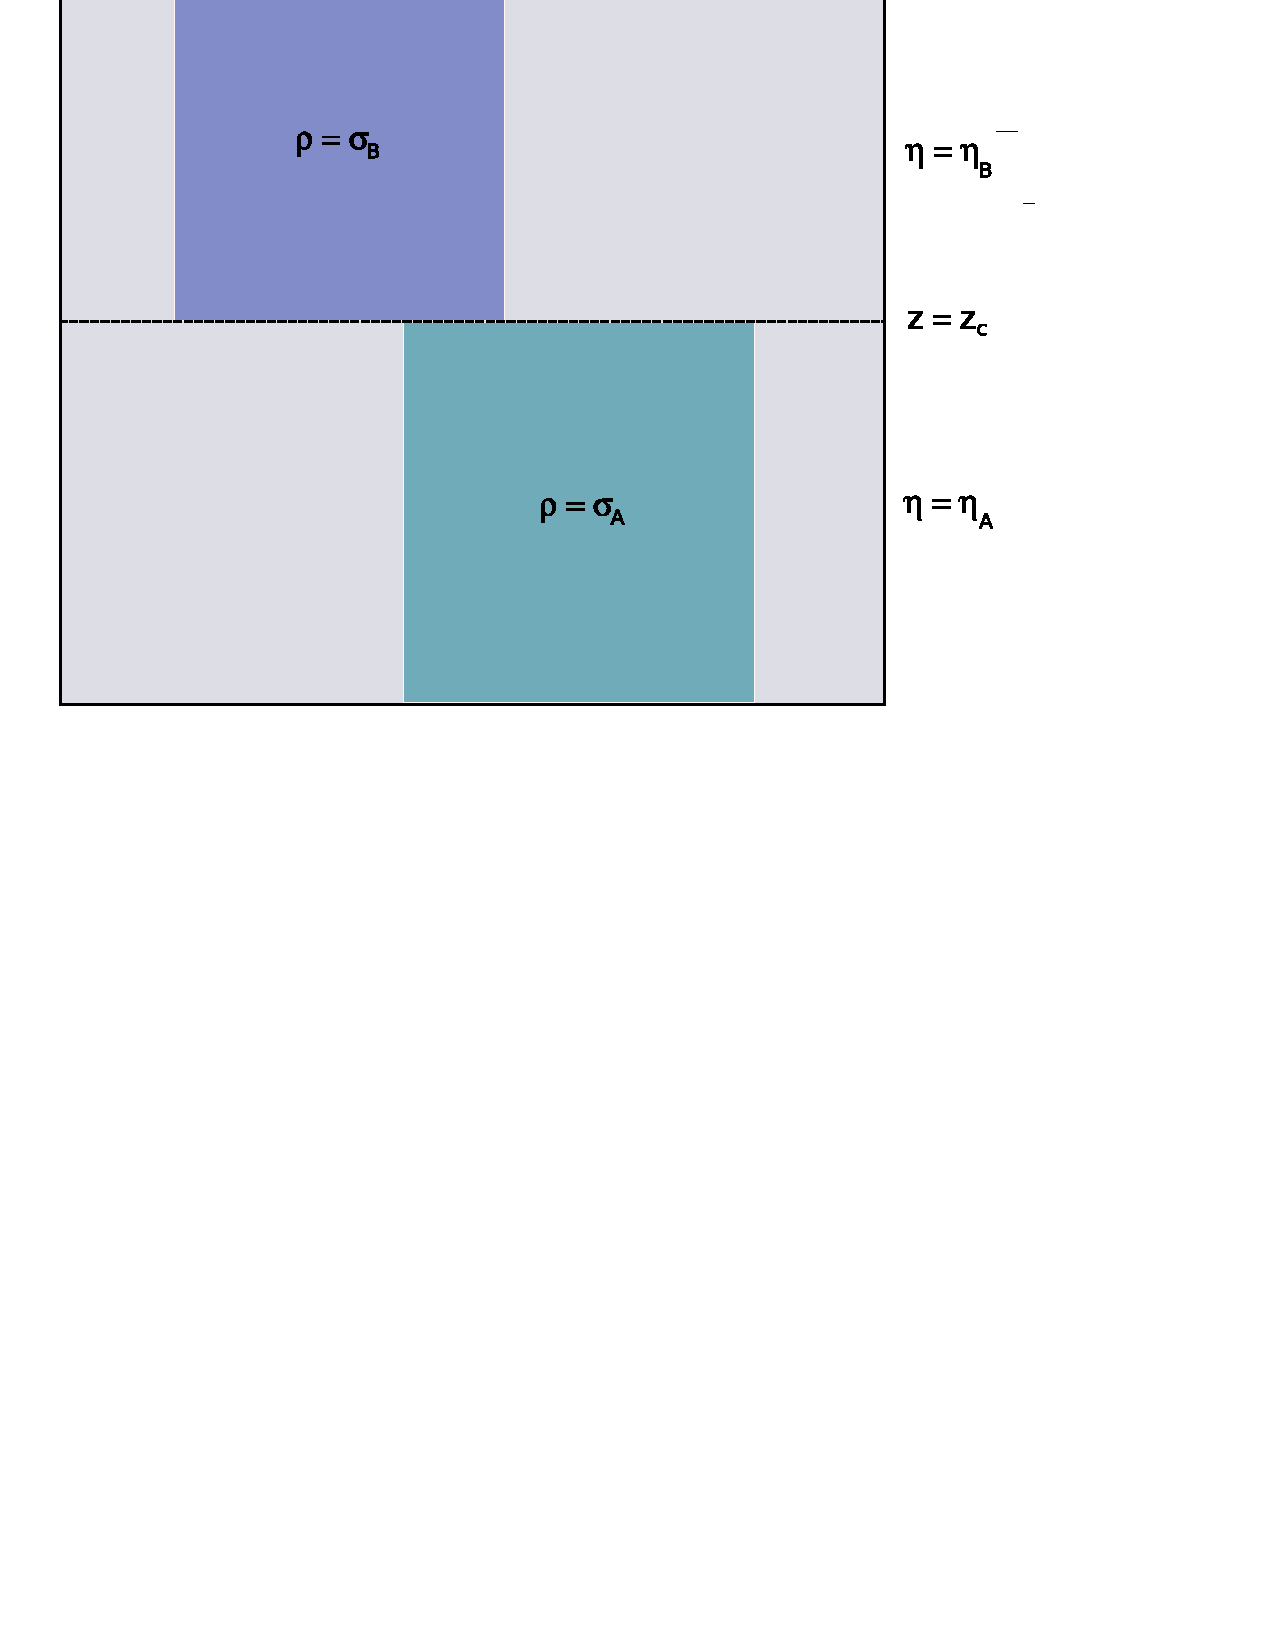
\includegraphics[width=6cm,clip]{../figs/figJ.pdf}
    \caption[Short caption]{\label{figJ} 
      Solution ({\bf SolJ}):
      This solution has a block of density $\rho = \sigma_B$ from $x_{0B}-dx_B/2 < x < x_{0B}+dx_B/2$ above
      $ z= z_c$ and a block of density $\rho = \sigma_A$ from $x_{0A}-dx_A/2 < x < x_{0A}+dx_A/2$ below
      $ z= z_c$.
      The viscosity is layered with a jump at $ z=z_c $.
      The boundary conditions are free slip everywhere on the surfaces of the unit box.}
  \end{SCfigure} 
  

